% This section may be divided by subheadings. Authors should discuss
% the results and how they can be interpreted in perspective of
% previous studies and of the working hypotheses. The findings and
% their implications should be discussed in the broadest context
% possible. Future research directions may also be highlighted.

\section{Discussion}

% This section may be divided by subheadings. Authors should discuss
% the results and how they can be interpreted in perspective of
% previous studies and of the working hypotheses. The findings and
% their implications should be discussed in the broadest context
% possible. Future research directions may also be highlighted.

%%%%%%%%%%%%%%%%%%%%%%%%%%%%%%%%%%%%%%%%%%

The goal of ROSMOD is to be a model-driven, component-based rapid
development, deployment, and experimentation toool suite for
distributed CPS.  This goal has been the driving force since the
beginning of ROSMOD during the 2014-2015 NASA SLI competition with the
AGSE.  ROSMOD itself was developed alongside the AGSE and in concert
with it; as we added features to the modeling language, the user
interface, or the generation and deployment infrastructure, we
immediately tested them with the AGSE.  The focus on the development
was always model-driven engineering coupled with component-based
software design principles enabling an iterative development cycle for
both the AGSE and ROSMOD.  Because of the competition's deadlines, we
focused on developing the AGSE and ROSMOD through short cycles between
design, implement, test, iterate.  These deadlines helped focus the
core of ROSMOD's architecture towards one of rapid system design,
development, and deployment.

Through this development cycle, our team had to maintain a balance
between many (sometimes conflicting) design considerations:

\begin{itemize}
\item utilizing component-based design to parallelize the development
  effort into subunits among each member
\item evolution of the design in concert with evolution of the
  implementation: must prototype and test quickly, but the
  implementation should be usable for the next phase of the design.
\item track and plan for materials lead-time, and testing/integration time
\item tool support, i.e. mechanical facilities and software
  development/testing support
\item expertise required for each component/subsystem design,
  development, and testing
\item importance of meaningful feedback especially with respect to
  errors and failures in software/hardware.
\end{itemize}

As in any software or hardware development, bugs and failures were
encountered in the development of both the AGSE hardware and software.
However, the use of the ROSMOD infrastructure allowed the causes of
those issues to be narrowed down and more quickly resolved.  For
example, the logging and tracing framework of ROSMOD enabled the
resolution of issues stemming from slow processor speed leading to
long execution times.  By using the logging and plotting features of
ROSMOD to trace the execution time of the component operations in the
AGSE software, we were able to determine that the NVIDIA Jetson was
running sub-optimally, and confirmed that the CPU frequency governor
was configured by default to dramatically throttle the main ARM cores
of the processor.  Furthermore, we were able to use the logging
framework to show that for some of the client-server connections in
the AGSE that were configured to be persistent connections, the
connection would drop immediately after being established.  After
determining this from the trace logs, we reconfigured those
client-server connections to no longer be persistent so they would
reconnect when required.

One of the main benefits from this timing and performance logging
infrastructure was the ability to validate the periodicity of timer
interactions in the AGSE.  By running the AGSE software and tracking
how long each operation takes, we were able to determine that the
original configuration of the AGSE timers was too frequent and needed
to be reduced by a factor of four.  By specifying deadlines on the all
the operations (esp. timer, server, and subscriber) we were able to
determine the bottlenecks in the system and figure out what parts of
the system had deadline violations (i.e. their execution times
exceeded their periodicity) and re-adjust the timers accordingly.

Figure \ref{fig:ExecPlot-armTimer} shows the execution time plot of the \emph{armTimer\_operation} in the high-level controller component. For sake of brevity, we avoid showing all the operational plots. In the context of Figure \ref{fig:AGSE}, this timer operation represents the execution of the high-level control state machine. The high-level controller communicates with multiple components over its life-span orchestrating various parts of the overall state machine e.g. initialization, sample detection, payload bay detection etc. Choosing an optimal period for this timer is necessary for many reasons. Firstly, the ROSMOD component operation scheduling is a non-preemptive one i.e. an operation must run to completion before the next request is serviced from the component operation queue. This means that if the timer operation does not complete before its period, the number of waiting requests in component queue start to monotonically rise. This hurts the system as a whole since subsequent requests take longer to complete and the high-level control breaks down. Secondly, inside the timer operation, the controller requires the services of both the motor control and the imaging components, often times via synchronous blocking interactions. This is the second cause of a potential problem as the blocking times are non-deterministic and dependent on the execution state of other embedded boards. For this reason, the AGSE software was deployed and experimented with to identify the optimal period where the response times are manageable. As shown in Figure \ref{fig:ExecPlot-armTimer}, the high-level controller has two set of spikes in execution time. The first set (between 100 and 150 seconds into the experiment), as confirmed by Figure \ref{fig:ExecPlot-sample-Bay-DetectionStateFromImageServer} corresponds to sample detection. The second set of spikes, between 200 and 250 seconds, is the payload bay detection. These plots quickly present the performance of the high-level controller and the worst-case response times during periodic image processing. 

\begin{figure}[t]
	\centering
	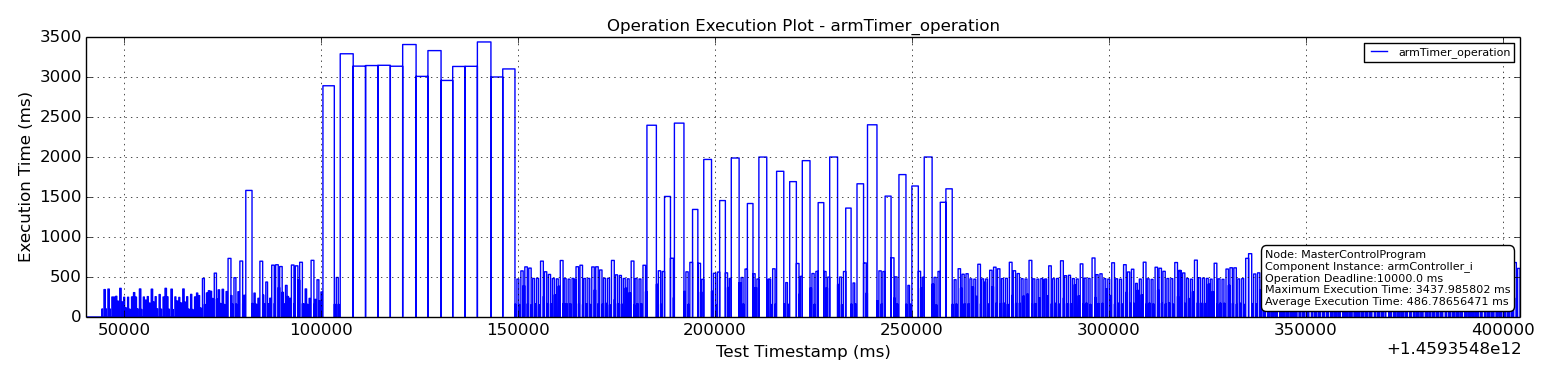
\includegraphics[width=\linewidth]{Figures/ExecPlot-armTimer.png}
	\caption{High-level Timer Execution}
	\label{fig:ExecPlot-armTimer}	
\end{figure}

\begin{figure}[t]
	\centering
	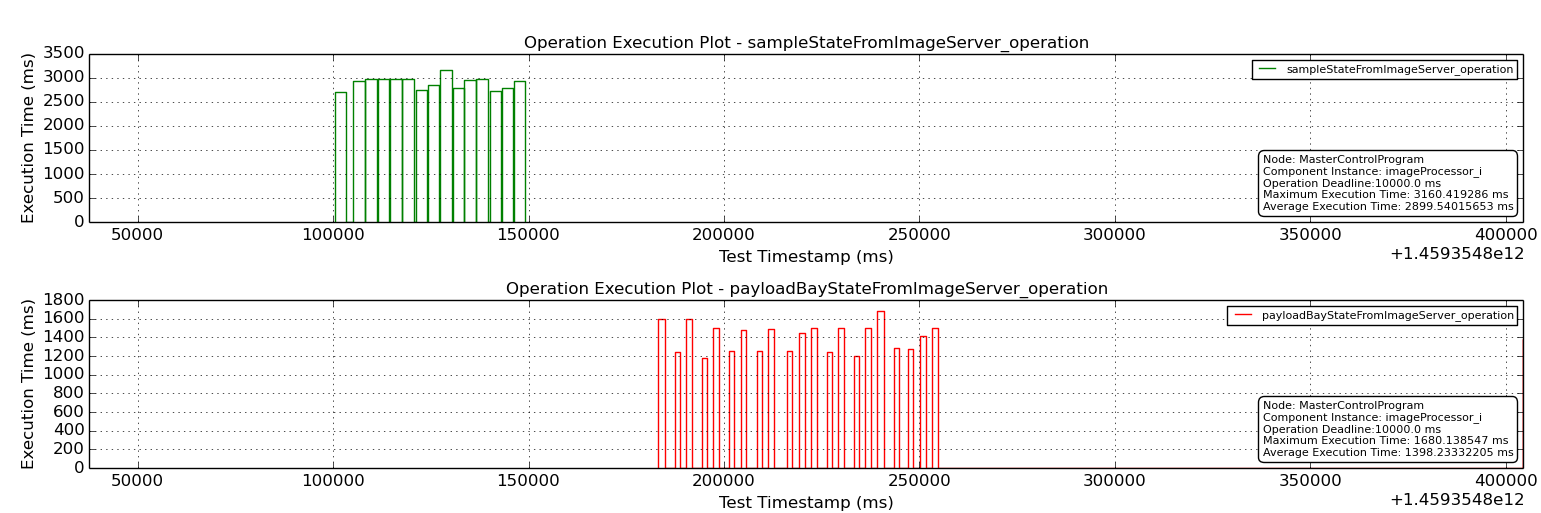
\includegraphics[width=\linewidth]{Figures/ExecPlot-sample-Bay-DetectionStateFromImageServer.png}
	\caption{Sample and Payload bay Detectors Execution}
	\label{fig:ExecPlot-sample-Bay-DetectionStateFromImageServer}	
\end{figure}

Figure \ref{fig:ExecPlot-sample-Bay-DetectionStateFromImageServer} presents the performance of the \emph{GetSampleState\_Server} and the \emph{GetPayloadState\_Server} in Figure \ref{fig:AGSE}. These servers are periodically invoked by the high-level controller during its operation, first during sample detection and then during payload bay detection. Each of these servers, on demand, are required to obtain the current camera feed from the Camera component, perform image processing, and return the results to the high-level controller. Thus, the interaction and data flow path is as follows: During sample detection, the high-level controller is periodically triggered to ask the Image Processor component to provide a new result. The Image Processor, in turn, queries the Camera component for a feed update. The Camera \emph{ImageServer}, as shown in Figure \ref{fig:ExecPlot-captureImage} responds to the Image Processor component with a new feed. This image server is also responding to the userDisplay component that receives the camera feed to display to the user. 

\begin{figure}[t]
	\centering
	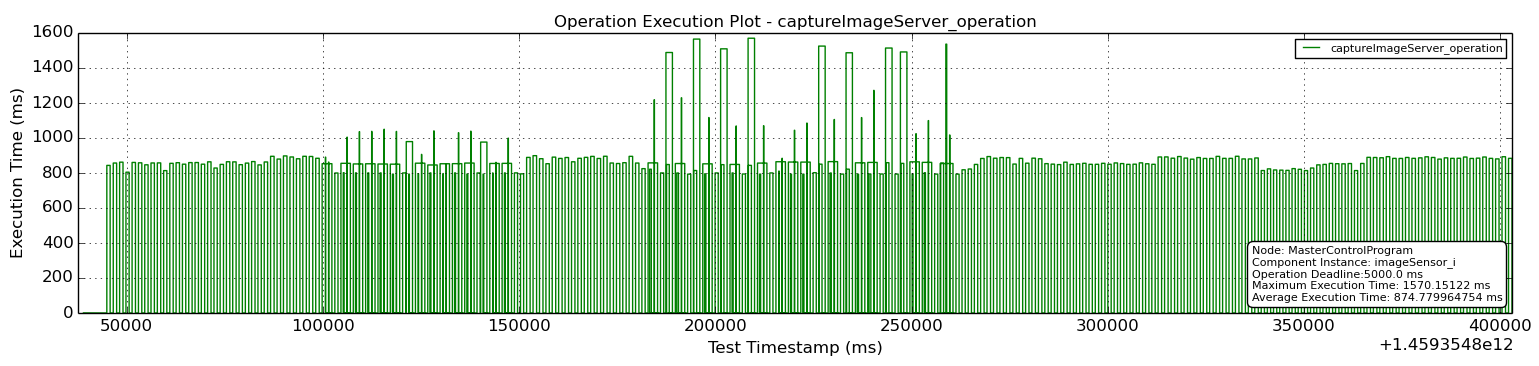
\includegraphics[width=\linewidth]{Figures/ExecPlot-captureImage.png}
	\caption{Camera Feed Reponse Times}
	\label{fig:ExecPlot-captureImage}	
\end{figure}

Wwe were able to use the ROSMOD deployment infrastructure to
quickly run separate experiments on the BeagleBone Blacks (single core
embedded computers), testing the performance impact of running our
motor control components in separate processes or as separate threads
in the same process.  By simply changing the deployment model and
re-running the same code we were able to get ROSMOD timing and
performance logs from the experiments to show the extra overhead of
process-level context switching on the single-core BeagleBone Black.

The use of ROSMOD's performance, timing, and trace logging (coupled
with the plotting utilities for those logs) enabled us to easily
visually verify the behavior and performance of the AGSE software or
spot anomalies when they occurred.  Furthermore, the use of
code-generation and automated build and deployment infrastructure
meant that far less code had to be inspected for errors when a
software or logical error cropped up, and the developers did not have
to spend time configuring or debugging the build and deployment
systems.  Finally, the use of a graphical modeling tool for specifying
the entire AGSE project from software to hardware to deployment
enabled faster training and communications between team members as
well as visual inspection of the software configuration, for instance
ensuring that all required components can respond to the user's
control inputs or verifying the other interaction patterns and
triggering operations for each component.

The rapid prototyping facilitated by ROSMOD and the ROS infrastructure
enabled the development of an overall \emph{smarter} robot. The
software requirements for autonomy were matched by the ROSMOD code
generators such that developers had to spend little time setting up
the build system and interaction patterns. The speed of development
was drastically improved and the \emph{business logic} code, i.e. the
core of the implementation of the system behavior, could be made more
robust in spite of the evolution of and inclusion of more autonomy.

\iffalse
Mention that the hardware for the robot was designed and developed
primarily by 2-4 people (dexter can decide) and the electronics and
software for the robot was designed and developed by 2 people, at the
same time that the ROSMOD toolsuite was developed.

Mention the pitfalls we encountered (w.r.t. using the logger to
realize the speed of the jetson, the client-server failure when
turning on persistent connections, the mechanical hardware, the
electrical hardware, lead time and shipping, model translation and
update from V0.3 to V1.0, etc.)
\fi
